% Filename  : samplepaper.tex
% Purpose   : A sample exam paper to demonstrate how to use the 'ditpaper'
%             TeX class.
% Author    : Emmet Caulfield
% Revision  : $Id: samplepaper.tex 2 2006-02-19 20:34:45Z emmet $
% Repository: $HeadURL: http://svn.netrogen.lan/tex-ditpaper/trunk/samplepaper.tex $
%

% 'nosolution' (default) and 'solution' toggle the inclusion of solutions
% in the output. The tag solution, below, is replaced by 'sed' 
% in the Makefile to cause both the paper and the solutions to be produced.
\documentclass[solution]{ditpaper}

\usepackage{epsf}
\usepackage{fleqn}
\usepackage{rotating}
\usepackage{graphicx}


%%%%%%%%%%%%%%%%%%%%%%%%%%%%%%%%%%%%%%%%%%%%
%% Start newcommand defs taken from aima slides style file %%%%%%%%%%%%%%
%%%%%%%%%%%%%%%%%%%%%%%%%%%%%%%%%%%%%%%%%%%%

\def\mysum{\begin{Huge}\mbox{$\Sigma$}\end{Huge}}
\def\myint{\begin{LARGE}\mbox{$\int$}\end{LARGE}}
\def\myprod{\begin{Huge}\mbox{$\Pi$}\end{Huge}}

\newcommand{\smbf}[1]{\mbox{{\smathbold #1}}}
\newcommand{\mbf}[1]{\mbox{{\bf #1}}}

%%%%%% logical symbols
\newcommand{\entails}{\models}
\newcommand{\implies}{\:\;{\Rightarrow}\:\;}
\newcommand{\textimplies}{\;{\Rightarrow}\;}
\newcommand{\impliessymbol}{\Rightarrow}
\newcommand{\lequiv}{\;\;{\Leftrightarrow}\;\;}
\newcommand{\textlequiv}{\;{\Leftrightarrow}\;}
\newcommand{\lequivsymbol}{\Leftrightarrow}
\newcommand{\xor}{\not\lequiv}
\newcommand{\All}[1]{\forall\,#1\;\;}
\newcommand{\Exi}[1]{\exists\,#1\;\;}
\newcommand{\Exii}[1]{\exists!\,#1\;\;}% -pnorvig
\newcommand{\Iot}[2]{\iota\,#1\,#2}
\newcommand{\Lam}[2]{\lambda #1\;#2}
\newcommand{\Qua}[3]{[#1\,#2\;#3]}

\newcommand{\union}{{\,{\cup}\,}}
\newcommand{\intersection}{{\,{\cap}\,}}
\renewcommand{\emptyset}{\{\,\}}
\newcommand{\emptylist}{[\,]}
\newcommand{\adjoin}[2]{\{#1|#2\}}
\newcommand{\elt}{{\,{\in}\,}}  %%%cuts down on spacing
\newcommand{\eq}{{\,{=}\,}}  %%%cuts down on spacing
\def\stimes{{\,\times\,}}       %%%cuts down on spacing

\newcommand{\sr}[1]{\mathrel{\raisebox{-0.6ex}{$\stackrel{#1}{\longrightarrow}$}}}
\newcommand{\srbox}[1]{\sr{\fboxsep=1pt\fbox{$\,{\scriptstyle #1}\,$}}}
\newcommand{\srboxbox}[1]{\sr{\fboxsep=1pt\fbox{\fbox{$\,{\scriptstyle #1}\,$}}}}

\def\Diff{\mbox{{\it Diff}}}

%%%%%% probability and decision theory
\newcommand{\pv}{\mbf{P}}
\newcommand{\qv}{\mbf{Q}}
\newcommand{\given}{\mid}
\def\transition#1#2{q(#1\rightarrow #2)}
\newcommand{\otherthan}{\overline}
\newcommand{\Parents}{Parents}
\newcommand{\parents}{parents}
\newcommand{\Children}{Children}
\newcommand{\children}{children}
\newcommand{\MarkovBlanket}{MB}
\newcommand{\markovBlanket}{mb}

\def\X{\mbf{X}}
\def\x{\mbf{x}}
\def\sx{\smbf{x}}
\def\Y{\mbf{Y}}
\def\y{\mbf{y}}
\def\sy{\smbf{y}}
\def\E{\mbf{E}}
\def\e{\mbf{e}}
\def\D{\mbf{D}}
\def\d{\mbf{d}}
\def\sbe{\smbf{e}}
\def\sE{\smbf{E}}
\def\T{\mbf{T}}
\def\O{\mbf{O}}
\def\se{\smbf{e}}
\def\Z{\mbf{Z}}
\def\z{\mbf{z}}
\def\sz{\smbf{z}}
\def\F{\mbf{F}}
\def\f{\mbf{f}}
\def\A{\mbf{A}}
\def\B{\mbf{B}}
\def\C{\mbf{C}}
\def\b{\mbf{b}}
\def\m{\mbf{m}}
\def\I{\mbf{I}}
\def\H{\mbf{H}}
\def\zeroes{\mbf{0}}
\def\ones{\mbf{1}}
\def\ev{\mbf{ev}}
\def\fv{\mbf{ev}}
\def\sv{\mbf{sv}}

%%%%%%%%%%%%%%%%%%%%%%%%%%%%%%%%%%%%%%%%%%%%
%% End newcommand defs taken from aima slides style file %%%%%%%%%%%%%%
%%%%%%%%%%%%%%%%%%%%%%%%%%%%%%%%%%%%%%%%%%%%





% These must be set or bizarre defaults will be used:
\facility{Kevin Street, Dublin 8}
\course{BSc. (Hons) in Computer Science}
\examcode{S249/401C}
\stage{Stage 4}
\session{Semester 2 Examinations 2011/2012}
\title{Artificial Intelligence II}
\examiners{Dr. John Kelleher\\
Dr. Deirdre. Lillis\\
Mr. Ray Walshe}
\examdate{Monday\\$14^{th}$ May 2012}
\examtime{\centerline{4:00 p.m to 6:00 p.m}}
\instructions{Question 1 is \textbf{compulsory}\par{} Answer Question 1 (40 marks) \textbf{and}\par{} any 2 Other Questions (30 marks each).}

\begin{document}


%aima chapters 18
% inductive bias, learning theory - supervised/unsupervised, overfitting, lazy/eager learner, classification v regression, false positive v false negatives, linear separability, consistency, evaluation

\question
\begin{enumerate}
	\item Explain what is meant by \textbf{inductive learning}.
	\marks{5}
	\begin{answer}
		Inductive Learning involves the process of learning by example � where a system tries to induce a general rule from a set of observed instances
	\end{answer}
	\item For some data sets it is possible to devise multiple hypotheses that are consistent with the data. Describe a heuristic for choosing among multiple consistent hypotheses and explain why your heuristic is reasonable.
		\marks{5}
\begin{answer}
One answer is to use Occam�s razor (sometimes called Ockham�s razor) : prefer the hypothesis that maximizes a combination of simplicity and consistency with the data. This makes sense, because hypotheses that are no simpler than the data themselves are failing to extract any pattern from the data. Defining simplicity is not easy but it seems reasonable to say that a degree-1 polynomial is simpler than a degree-12 polynomial.
\end{answer}	
	\item Describe the differences between \textbf{lazy learners} and \textbf{eager learners}, giving examples of each.
			\marks{10}
		\begin{answer}
			Definitions:
			\begin{description}
				\item [Lazy learners] do not try to build a model from the training data, but simply use it at classification time
				\item [Eager learners] build a mode from the training data during training, and use only this model at classification time, ignoring the original data.
			\end{description}
			Key differences:
			\begin{itemize}
				\item Lazy methods may consider query instance when deciding how to generalise beyond the training data D; eager methods cannot since they have already chosen global approximation when seeing the query.
				\item \textbf{Efficiency} lazy learners require less training times but more time at prediction; eager learners require more training times by less time for prediction
				\item \textbf{Accuracy} lazy learners effectively uses a richer hypothesis space since it uses many local linear functions to form its implicit global approximation to the target function; eager learners must commit to a single hypothesis that covers the entire instance space.
				\item It is easier for lazy learners to handle \textbf{concept drift}
			\end{itemize}
			Examples:
			\begin{description}
				\item [Lazy learning example]: case based reasoning
				\item [Eager learning example]: Decision=tree, neural networks, support vector machines
			\end{description}
		\end{answer}
	\item Let us say we have three classification algorithms. How can we order these three from best to worst?
	\marks{20}
	\begin{answer}
		This is a discursive question so giving a precise answer is not appropriate. However, key points that the student should touch on include:
		\begin{itemize}
		\item Predictive accuracy
		\item Speed and scalability 
		\begin{itemize}
			\item Time to construct the model
			\item Time to use the model
		\end{itemize}
		\item Robustness (handling noise and missing values)
		\item Scalability
		\item Interpretability (understanding and insight provided by the model)
	\end{itemize}
	It should be noted also, that these evaluation criteria are application dependent.
	\end{answer}
\end{enumerate}


\newpage

%Q2
% knn and CBR 
% information theory, entropy, Decision Trees, Inductive logic programming

\begin{table}[htdp]
\caption{Class Exam Results: a 1 indicates the student possesses the feature listed in the column and 0 indicates that they do not. The final column lists whether or not the student was awarded a $1^{st}$ this year}
\begin{center}
\begin{tabular}{|c|c|c|c|c|}
\hline
Student & $1^{st}$ last year & Works hard? & Blonde  & $1^{st}$ this year \\
\hline
X & 1 & 1 & 0 & 1\\
Y & 0 & 1 & 1 & 0\\
Z & 0 & 1 & 0 & 0\\
\hline
\end{tabular}
\end{center}
\label{tab:class-results}
\end{table}%

\begin{table}[htdp]
\caption{The attributes of the student whose script was not marked. A 1 indicates the student possesses the feature listed in the column and 0 indicates that they do not. The column on the right contains a ? because they have not been graded yet.}
\begin{center}
\begin{tabular}{|c|c|c|c|c|}
\hline
Student & $1^{st}$ last year & Works hard? & Blond  & $1^{st}$ this year \\
\hline
U & 1 & 0 & 0 & ?\\
\hline
\end{tabular}
\end{center}
\label{tab:stu-atts}
\end{table}%
			
\question 
	\begin{enumerate}
			\item Discuss the advantages and disadvantages of \textbf{\textit{k}-Nearest Neighbour} classification.
				\marks{5}
				\begin{answer}
				Strengths
				\begin{enumerate}	
					\item No training involved  lazy learning
					\item New data can be added on the fly
					\item Some explanation capabilities
					\item Robust to noisy data by averaging k-nearest neighbors
				\end{enumerate}
				Weaknesses
				\begin{enumerate}
					\item Not the most powerful classification (generally its accuracy will be lower than an ANN or SVM model)
					\item Slow classification 
					\item Curse of dimensionality (as you increase the number of features you need more and more examples to cover the problem space - kNN are particularly susceptible to this issue as they do not do any feature selection).
				\end{enumerate}
			\end{answer}	
		\item Just before an exam board a lecturer finds an exam script by student $U$ that the lecturer had forgotten to mark. The lecturer does not have time to correct the script before the exam board, so they decide to use a nearest-neighbour approach to decide whether or not to award student $U$ a $1^{st}$. The case base of results the lecturer used is listed in Table \ref{tab:class-results} and the attributes of student $U$ are listed in Table \ref{tab:stu-atts} .
				\begin{enumerate}
					\item Assuming the lecturer uses Euclidean distance 
								\begin{center}
								$d(x_1,x_2)=\sqrt{\sum_{r=1}^{n} (a_r(x_1) - a_r(x_2))^2}$
								\end{center}
								 as their distance metric, compute the distance between the  student $U$ and each of the students in the case base.
			  \marks{5}
				\begin{answer}
					\begin{center}
						\begin{tabular}{|c|c|c|c|c|c|}
						Student & $1^{st}$ last year & Works hard? & Blond  & $1^{st}$ this year & Distance \\
						\hline
						X & 1 & 1 & 0 & 1 & 1.00\\
						Y & 0 & 1 & 1 & 0 & 1.732\\
						Z & 0 & 1 & 0 & 0 & 1.414\\
						\hline
						\end{tabular}
					\end{center}
				\end{answer}
			\item Given that the lecturer used \textbf{\textit{1}-NN} classification was student $U$ awarded a $1^{st}$?
				\marks{5}
				\begin{answer}
				Using Euclidean distance as a measure of distance student $X$ is the closest instance in the case base to student $U$. Consequently, using $1-NN$ classification student $U$ would be awarded the same result as student $X$. So student $U$ would be awarded a $1^{st}$
				\end{answer}
			\item If the lecturer used \textbf{\textit{3}-NN} classification would student $U$ be awarded a $1^{st}$?
				\marks{5}
				\begin{answer}
				If the lecturer used $3-NN$ all the instance in the database would be considered and the student would be awarded the most frequent occurring classification in the case base. In this instance, the student would not be awarded a $1^{st}$ because two out of the three students in the case base were not awarded $1^{st}$s. 
				\end{answer}
		\end{enumerate}
		% Information theory and Decision Trees
		
		\item Table \ref{tab:classification-data}, on the next page lists a classification dataset. Each instance in the dataset has two explanatory attributes (attribute 1 and attribute 2) and is classified as either a positive (+) or a negative(-) example.		
				\begin{enumerate}
			\item Calculate the classification \textbf{entropy} for this dataset.
			\marks{5}
			\begin{answer}
				Entropy is $-\frac{3}{5}log_2\frac{3}{5}-\frac{2}{5}log_2\frac{2}{5}=0.971$
			\end{answer}
			\item Calculate the \textbf{information gain} for attribute 1 and attribute 2.
			\marks{5}
			\begin{answer}
				Entropy for attribute 1 = T $-\frac{3}{4}log_2\frac{3}{4}-\frac{1}{4}log_2\frac{1}{4}=0.811$\\
				Entropy for attribute 1 = F $0-\frac{1}{1}log_2\frac{1}{1}=0$\\
				Gain for attribute 1 $0.971-(\frac{4}{5}\times0.811+\frac{1}{5}\times0)=0.322$\\
				Entropy for attribute 2 = T $-\frac{2}{3}log_2\frac{2}{3}-\frac{1}{3}log_2\frac{1}{3}=0.918$\\
				Entropy for attribute 2 = F $-\frac{1}{2}log_2\frac{1}{2}-\frac{1}{2}log_2\frac{1}{2}=1.0$\\
				Gain for attribute 2 $0.971-(\frac{3}{5}\times0.918+\frac{2}{5}\times1)=0.02$\\
			\end{answer}
		\end{enumerate}
	\end{enumerate}

\newpage

			\begin{table}[htb]
			\begin{center}
			\begin{tabular}{|c|c|c|}
				Attribute 1 & Attribute 2 & Classification \\
				\hline
				T & T & + \\
				T & F & - \\
				T & F & + \\
				T & T & + \\
				F & T & - \\
			\end{tabular}
			\end{center}
			\caption{Classification Dataset}
			\label{tab:classification-data}
		\end{table}


\newpage
	
%Q3 30 marks
% basic probability 5
% bayesian networks 10
% bayesian learning  15
\begin{table}[htb]
\caption{Full joint distribution for a dentist visit}
\begin{center}
\begin{tabular}{c|c|c|c|c|}
                          & \multicolumn{2}{c}{$toothache$} \vline & \multicolumn{2}{c}{$\lnot toothache$}  \vline \\
\hline
                          & $catch$ & $\lnot catch$ & $catch$ & $\lnot catch$ \\
 $cavity$          & 0.108     & 0.012             & 0.072      & 0.008             \\
 $\lnot cavity$ & 0.016     & 0.064             & 0.144      & 0.576             \\
\end{tabular}
\end{center}
\label{tab:fjd}
\end{table}%

\begin{figure}
	\begin{center}
	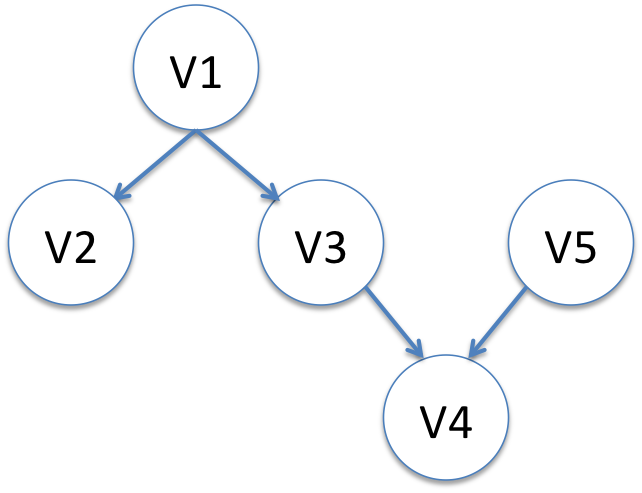
\includegraphics[width=2.5in]{./images/callan-chap5-q4.png}
	\end{center}
	\caption{An example Bayesian network.}
	\label{fig:callan-ch5-q4}
\end{figure}


\question
	\begin{enumerate}
		%basic probability
		\item Given the full joint distribution shown in Table \ref{tab:fjd}, calculate $\textbf{P}(Toothache|cavity)$.
					\marks{5}
					\begin{answer}
						This asks for the vector of probability values for $Toothache$, given that $Cavity$ is true.\\
						 $P(Toothache|cavity ) = \langle\frac{0.108 + .012}{0.2}, \frac{0.072 + 0.008}{0.2}\rangle = \langle 0.6, 0.4\rangle$ 
					\end{answer}

		%bayesian networks
		\item Express the joint probability distribution for the Bayesian network shown in Figure \ref{fig:callan-ch5-q4} using the chain rule.
			\marks{10}
			\begin{answer}
				The chain rule is: 
				\begin{center}
							$P(x_1,\ldots,x_n) = \prod_{i=1}^n P(x_i | x_{i-1}, \dots , x_1)$
				\end{center}
				In a properly constructed bayesian network: 
				\begin{center}$
					\parents(X_i) \subseteq \{ x_{i-1}, \dots, x_1 \}
				$\end{center} 
				Therefore, in a properly constructed Bayesian network: 
				\begin{center}$
					P(x_1,\ldots,x_n) = \myprod_{i\eq 1}^n P(x_i | x_{i-1}, \dots , x_1) = \myprod_{i\eq 1}^n P(x_i|\parents(X_i))
				$\end{center} 
				So the joint probability distribution for the given network is: 
				\begin{center}$
					P(V4|V3, V5)P(V3|V1)P(V2|V1) P(V5)P(V1)
				$\end{center} 
			\end{answer}

		%bayesian learning
		\item Consider the following time keeping patterns of the lecturers in your college:
		\begin{itemize}
			\item 25\% of lecturers start 75\% of their lectures on time and 25\% late.
			\item 50\% of lecturers start 50\% of their lectures on time and 50\% late.
			\item 25\% of lecturers start 25\% of their lectures on time and 75\% late.
		\end{itemize}
		\begin{enumerate}
		\item Given that both the $1^{st}$ and $2^{nd}$ Artificial Intelligence lectures of the year started on time, compute the posterior probability that your Artificial Intelligence lecturer follows each of the three time keeping patterns.
		\marks{10}
		\begin{answer}
			To begin we will define some notation. Let: 
			\begin{itemize}
				\item $h_1$ denote the hypothesis that your AI lecturer starts 75\% of their lectures on time $P(h_1)=0.25$.
				\item $h_2$ denote the hypothesis that your AI lecturer starts 50\% of their lectures on time $P(h_2)=0.50$.
			   	\item $h_3$ denote the hypothesis that your AI lecturer starts 25\% of their lectures on time $P(h_3)=0.25$.
			\end{itemize}
			Also, if we use the notation $ontime_x$ to represent the observation that a lecture x started on time, then the probability of any given AI lecture starting on time given a particular hypothesis $h$ is:
			\begin{itemize}
				\item $P(ontime_x|h_1)=0.75$ .
				\item $P(ontime_x|h_2)=0.50$ .
				\item $P(ontime_x|h_3)=0.25$ .
			\end{itemize}
			Then:
			\begin{itemize}
				\item By Bayes' rule, we can compute the posterior probability of a hypothesis given the data so far using: 
				\begin{center}
					$P(h_i|\textbf{d}) = \alpha P(\textbf{d}|h_i) P(h_i)$
				\end{center}
				\item And, the likelihood of the data given a hypothesis is calculated using: 
				\begin{center}
					$P(\textbf{d}|h_i) = \prod_j P(d_j|h_i)$
				\end{center}
			\end{itemize}
			So:
			\begin{itemize}
				\item $P(h_1|ontime_1,ontime_2)=\alpha (\prod_{j=1}^2 P(ontime_j|h_1))P(h_1)=\alpha 0.75^2 \times 0.25=\alpha 0.375=\frac{0.375}{1.0} = 0.375$.
				\item $P(h_2|ontime_1,ontime_2)=\alpha (\prod_{j=1}^2 P(ontime_j|h_2))P(h_1)=\alpha 0.50^2 \times 0.50=\alpha 0.500=\frac{0.500}{1.0} = 0.500$.
				\item $P(h_3|ontime_1,ontime_2)=\alpha (\prod_{j=1}^2 P(ontime_j|h_3))P(h_1)=\alpha 0.25^2 \times 0.25=\alpha 0.125=\frac{0.125}{1.0} = 0.125$.
			\end{itemize}
		\end{answer}
		\item Given that both the $1^{st}$ and $2^{nd}$ Artificial Intelligence lectures of the year started on time, what is the Bayesian Prediction that the $3^{rd}$ Artificial Intelligence lecture will start on time? 
			\marks{5}
		\begin{answer}
			Bayesian predictions use a likelihood-weighted sum over the hypotheses: 
			\begin{center}
				$P(X|\textbf{d})=\sum_i P(X|h_i)P(h_i|\textbf{d})$
			\end{center}
			In this instance we get:
			\begin{eqnarray*}
				P(ontime_{3}|\textbf{d})&=&\sum_i P(ontime_{3}|h_i)P(h_i|\textbf{d})\\
				&=& (0.75 * 0.375) + (0.5 * 0.5) + (0.25 *0.125)\\
				&=& 0.28125 + 0.25 + 0.03125\\
				&=& 0.5625			
			\end{eqnarray*}
		\end{answer}
		\end{enumerate}
	\end{enumerate} %end Q3

%
\newpage

%Q4
%Linear Regression Neural Nets, SVMs, Ensemble Learning

\begin{table}
\begin{center}
\begin{tabular}{ccccc}
\hline
x & 2 & 4 & 6 & 8\\
\hline
y & 2 & 5 & 5 & 8\\
\hline
\end{tabular}
\caption{Example Dataset for Linear Regression Question}
\label{tab:linregTab1}
\end{center}
\end{table}

\question 
	\begin{enumerate}
		%Regression Learning
		\item Assuming a domain with one explanatory variable $x$ and one dependent variable $y$ linear regression uses the following formula to model the relationship between the explanatory and dependent variable: 
	\begin{center}
		$f(x) = w_1x + w0$
	\end{center}
where $w1$ and $w0$ are computed using the following formulae (where $M$ is number of data points in the dataset):
	\begin{large}
		\begin{center}
		$w_1 =  \frac{(M \sum_{i=1}^M x_i y_i) - (\sum_{i=1}^{M} x_i \sum_{i=1}^{M} y_i)} {(M \sum_{i=1}^{M} x_i^2) - (\sum_{i=1}^{M} x_i)^2}$
	\end{center}
	\begin{center}
		$w_0 = (\frac{1}{M} \sum_{i=1}^{M} y_i) - (\frac{w_1}{M} \sum_{i=1}^{M} x_i)$
	\end{center}
	\end{large}
Using the data in Table \ref{tab:linregTab1} compute the values of $w_0$ and $w_1$ that provide the best linear fit to the data.
			\marks{10}
			\begin{answer}
				First we need to compute the values of the equation components:
			\begin{itemize}
				\item M = 4
				\item $\sum_{i=1}^{M} x_i y_i = 4 + 20 + 30 + 64 = 118$
				\item $\sum_{i=1}^{M} x_i = 2 + 4 + 6 + 8 = 20$
			   	\item $\sum_{i=1}^{M} y_i = 2 + 5 + 5 + 8 = 20$
			  	\item $\sum_{i=1}^{M} x_i^2 = 4 + 16 + 36 + 64 = 120$
			  	\item $(\sum_{i=1}^{M} x_i)^2 = 20^2 = 400$
			\end{itemize}
				Given these values,  $w_1$:
				\begin{center}
					\textbf{$w_1= \frac{(4*118)-(20*20)}{(4*120)-400} = \frac{72}{80}=0.9$}
				\end{center}
				And, $w_0$:
				\begin{center}
				\textbf{$w_0= (\frac{1}{4}*20) - (\frac{0.9}{4}*20)= 5-4.5=0.5$}
			\end{center}
			\end{answer}		
		%Neural Nets	
		\item Figure \ref{fig:nn} shows a backprogation network that is currently processing the training vector $[1.0, 0.9, 0.9]$ that has an  associated target vector $[0.1, 0.9, 0.1]$. Given that the output from unit B is $0.6$ and from C is $0.8$, and assuming that the activation function used at all nodes in the network is the logistic function (i.e., $f(x) = \frac{1}{1 + \exp^{-x}}$): 
		\begin{enumerate}
			\item Calculate the actual output vector (to 3 decimal places).
			\marks{5}
			\begin{answer}
				Output of unit $i = f(\sum_{j=1}^{n}W_{j,i}\times activation_j)$\\
				First output unit input = -0.3 x 0.6 + 0.9 x 0.8 = 0.54 $\rightarrow$ f(0.54) = 0.632\\
				Second output unit input = -0.6 x 0.6 + -0.1 x 0.8 = -0.44 $\rightarrow$ f(-0.44) = 0.392\\
				Third output unit input = 0.4 x 0.6 + 1.2 x 0.8 = 1.2 $\rightarrow$ f(1.2)= 0.769\\
			\end{answer}
			\item Calculate the error for each output unit.
			\marks{5}
			\begin{answer}
				Error =  target - output\\
				First output unit = (0.1 - 0.632)  = - 0.532\\
				Second output unit = (0.9 - 0.392) = 0.508\\
				Third output unit = (0.1 - 0.769) = - 0.696\\
			\end{answer}
			\item Calculate the error for each hidden unit B and C.
			\marks{10}
			\begin{answer}
				Each hidden node $j$ is responsible for some fraction of the error $Err_i$ of each of the output units $i$ to which it connects. Thus the $Err_i$ values are divided according to the strengths of the connection between the hidden node and the output nodes and are propagated back to the hidden nodes. Where a hidden node feeds-forward into more than 1 output node the errors propagated back to it are summed: $Err_j = \sum_{i=1}^{n}W_{ji} \times Err_i$:
				$Err_{B} = (-0.3 \times -0.532) + (-0.6 \times 0.508) + (0.4 \times -0.696) = 0.1596 + -0.3048 + -0.2784 = -0.4236$\\
				$Err_{C} = (0.9 \times -0.532) + (-0.1 \times 0.508) + (1.2 \times -0.696) =  -0.4788 + -0.0508 + -0.8352  = -1.3648$\\
			\end{answer}		
		\end{enumerate}
	\end{enumerate}

\begin{figure}[htbp]
\begin{center}
\includegraphics[width=3.5in]{./images/nn_callan_q10_2.png}
\caption{Example Neural Net}
\label{fig:nn}
\end{center}
\end{figure}


\end{document}
